\chapter{Otevřená data a principy Linked Data}
\label{sec:kap2}

Předmětem této kapitoly je čtenáře stručně seznámit se základními pojmy a principy otevřených, propojitelných dat a následně s technologiemi sloužícími k jejich zápisu a zpracování.

\section{Otevřená data (Open Data)}

\textit{\uv{Open data can help us address the greatest challenges of our time and generate value for everyone}} - Open Data Institute 2012
\newline

Začneme definicí, kterou si postupně vysvětlíme. Jako otevřená data můžeme chápat údaje zveřejněná na internetu, která jsou\cite{mv}

\begin{enumerate}
\item úplná
\item snadno dostupná
\item strojově čitelná
\item používající standardy s volně dostupnou specifikací
\item zpřístupněna za jasně definovaných podmínek užití dat s minimem omezení
\item dostupná uživatelům při vynaložení minima možných nákladů
\end{enumerate}

\subsection*{Úplnost}

Pokud se rozhodneme zveřejňovat data, tak v případě, že nás neomezuje zákon, či jiná restriktivní opatření, měli bychom dbát na to, aby byla úplná, resp. v maximálním možné rozsahu. Není cílem zveřejňovat útržky ztrácející vypovídající hodnotu.

\subsection*{Snadná dostupnost}

Základní požadavek na dostupnost otevřených dat spočívá v tom, že by měla být k dispozici kdykoli, ne pouze např. na vyžádání. Otevřená data budou také přínosem pro širokou veřejnost jedině tehdy, pokud budou snadno dohledatelná. Skrytá data za změtí odkazů se hledají špatně.

\subsection*{Strojová čitelnost}

Klíčovou vlastností otevřených dat je strojová čitelnost. Otevřeným datům by měl porozumět nejen člověk, ale i stroj. Účelem je umožnit data automatizovaně zpracovávat, analyzovat, počítat statistiky apod.

\subsection*{Otevřené standardy}

Software, nástroje či metodiky potřebné k zpracování dat by měly být volně dostupné. Data v uzavřeném formátu, která potřebují ke zpracování konkrétní proprietární software, postrádají smysl otevřenosti.

\subsection*{Zpřístupněna za jasně definovaných podmínek}

Typicky je třeba dbát na to, aby data byla zveřejňována pod otevřenou licencí.\footnote{Více k problematice licencování a užití otevřených dat lze dohledat na webu Ministerstva vnitra\cite{mv}}

\subsection*{Dostupná uživatelům s minimem nákladů}

Je třeba si uvědomit, že nezveřejňujeme data pro data. Zveřejňujeme pro přidanou hodnotu, např. pro lepší službu nebo vyšší efektivitu. Náklady na zveřejnění by tak neměly přesáhnout případná zlepšení.
\newline

\begin{figure}[h]
\centerline{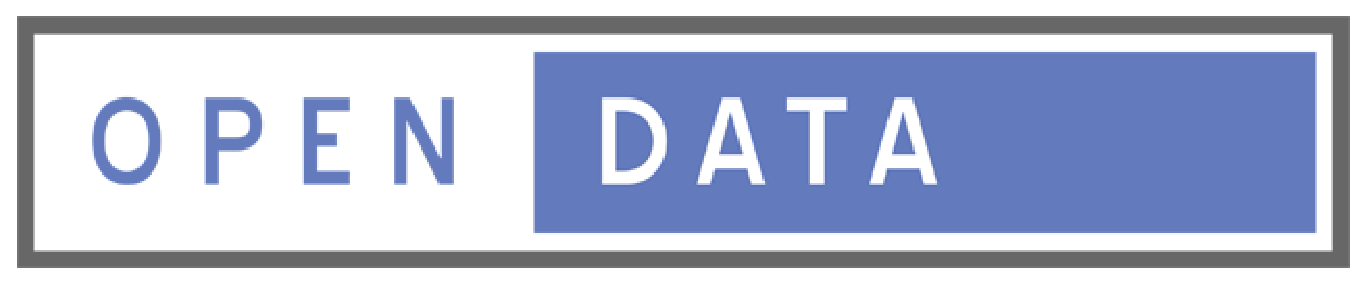
\includegraphics[width=100mm]{img/opendata.eps}}
\caption{Logo otevřených dat}
\label{modules}
\end{figure}

\newpage

\section{Kvalita otevřených dat}

Tvůrce WWW a ředitel konsorcia W3C Tim Berners-Lee navrhl pěti hvězdičkový systém, jak kategorizovat otevřená data (viz Obrázek \ref{obr:5star_steps}). Každá hvězdička definuje stupeň otevřenosti, kde 5$\bigstar$ znamená nejvyšší kvalitu dat, 1$\bigstar$ naopak nejmenší. Také platí, že každý stupeň je nadmnožinou (rozšířením) stupně předešlého.

\section{Stupně otevřenosti\protect\cite{5starInfo}}

\subsection*{$\bigstar$ Libovolná zveřejněná data pod otevřenou licencí}

\medskip

\begin{itemize}
\item Přínosy pro uživatele - uživatel může data číst, tisknout, ukládat, přenášet, měnit a sdílet podle svého uvážení
\item Přínosy/náklady pro vydavatele - velmi nenáročné na publikaci
\item Příkladem může být formát PDF
\end{itemize}

Publikace dat na úrovni 1$\bigstar$ je zdaleka nejjednodušší a nepotřebuje příliš vynaloženého úsilí. Určitě je lepší zveřejňovat data na úrovni 1$\bigstar$, než vůbec. Využitelnost dat však může být velmi obtížná, např. díky nutnosti dolování dat z PDF dokumentů.

\subsection*{$\bigstar\bigstar$ Strukturovaná data ve strojově čitelném formátu}

\medskip

\begin{itemize}
\item Přínosy pro uživatele - uživatel může pokročile zpracovávat data s využitím proprietárních nástrojů k tomu určených
\item Přínosy/náklady pro vydavatele - velmi nenáročné na publikaci
\item Příkladem může být formát MS Excel (.xls)
\end{itemize}

V dnešní době už poměrně rozšířený způsob publikace dat. Zpracování dat ale vyžaduje specifické nástroje k tomu určené. Pokud tedy chceme zpracovávat např. excelovskou tabulku (.xls), potřebujeme k tomu komerční produkt MS Excel\footnote{Toto se netýká formátu .xlsx. Ten již vychází z otevřené specifikace Office Open XML\cite{OOXML}. Data publikovaná v .xlsx formátu tedy můžeme chápat jako 3$\bigstar$.}. 

\subsection*{$\bigstar\bigstar\bigstar$ Formát dat je otevřený}

\medskip

\begin{itemize}
\item Přínosy pro uživatele - uživatel při zpracování dat není omezen žádným specifickým nástrojem
\item Přínosy/náklady pro vydavatele - nenáročné na publikaci, může však vyžadovat transformaci dat, např. z uzavřeného formátu
\item Příkladem může být formát CSV
\end{itemize}

Teprve v této kategorii se můžeme bavit o \uv{opravdových} otevřených datech. Resp. data musejí mít stupeň otevřenosti minimálně 3$\bigstar$ , aby naplnila základní definici otevřených dat uvedenou výše.

\subsection*{$\bigstar\bigstar\bigstar\bigstar$ Jednotlivé objekty jsou identifikovány pomocí URI}

\medskip

\begin{itemize}
\item Přínosy pro uživatele - uživatel se může na data odkazovat, odkazy si ukládat, případně data snadno kombinovat s jinými (na stejném, nebo vyšším stupni)
\item Přínosy/náklady pro vydavatele - náročnější na publikaci
\item Příkladem může být formát RDF
\end{itemize}

Důležité je dbát na to, aby URI nebylo virtuální, resp. aby se po dotázání uživateli vrátil požadovaný obsah. V prostředí WWW je zajištění obsahu typicky praktikováno skrze protokol HTTP. 

Díky URI identifikaci můžeme data reprezentovat jako orientovaný graf propojených objektů, které na sebe mohou vzájemně odkazovat. K popisu takovýchto dat se používá formát RDF.[\ref{sec:RDF}]  

V prostředí České republiky považováno jako nadstandard.

\subsection*{$\bigstar\bigstar\bigstar\bigstar\bigstar$ Data jsou propojena se souvisejícími daty}

\medskip

\begin{enumerate}
\item Přínosy pro uživatele - vytvoření efektu datové sítě, větší informační hodnota dat    
\item Přínosy/náklady pro vydavatele - náročnější na publikaci
\item Příkladem může být formát RDF
\end{enumerate}

V této nejvyšší kategorii se data mohou stát součástí datové sítě propojených grafů.

\begin{figure}[h]
\centerline{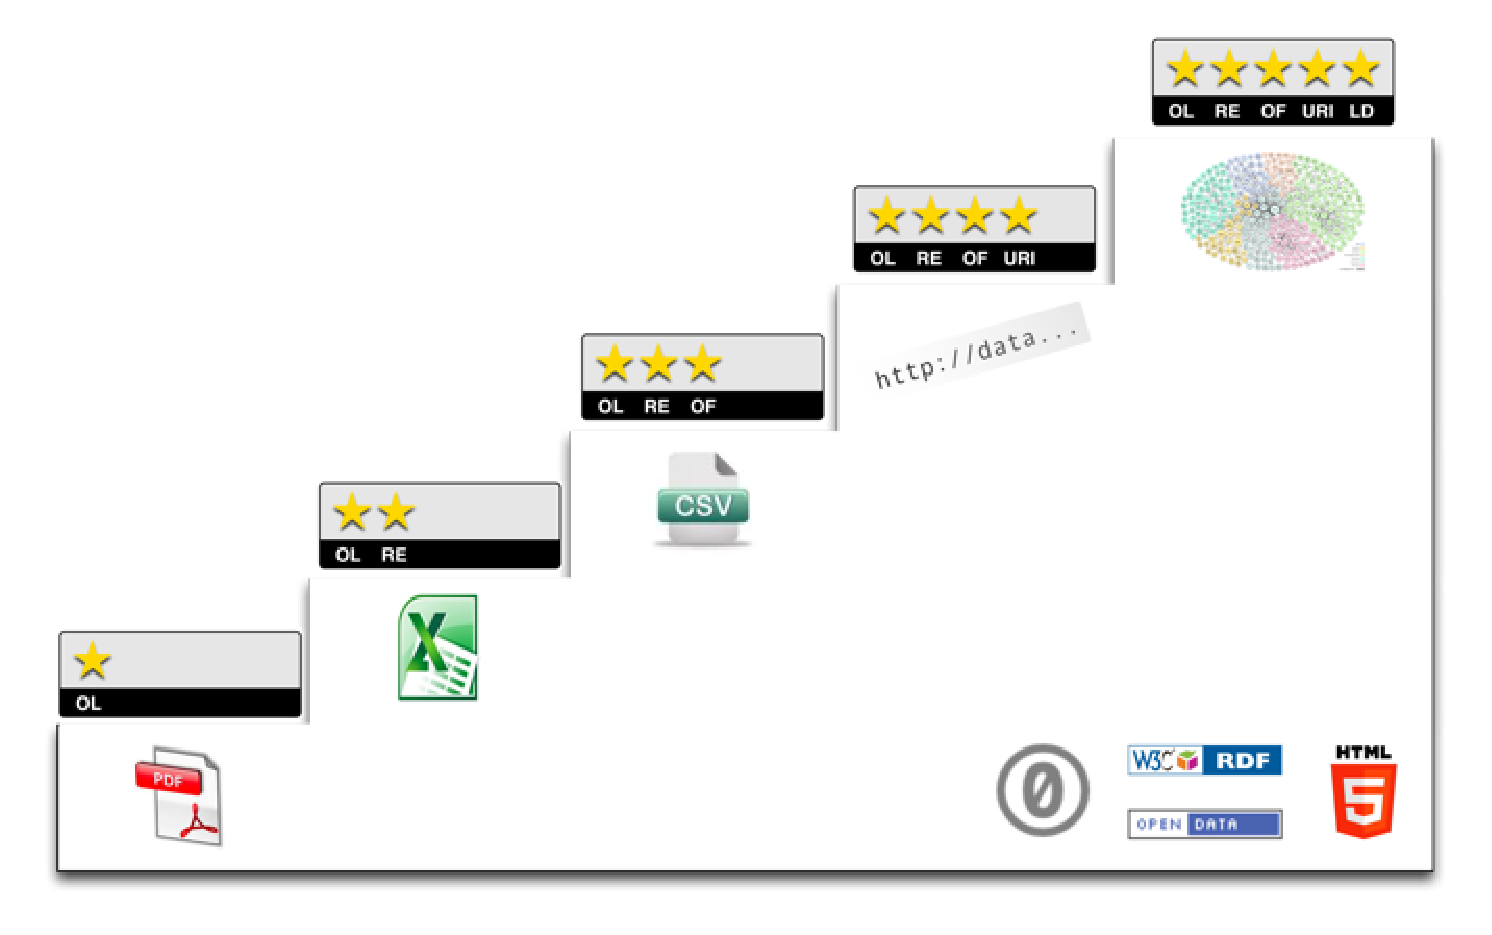
\includegraphics[width=\textwidth]{img/5star_steps.eps}}
\caption{Stupně otevřenosti dat}
\label{obr:5star_steps}
\end{figure}

\newpage

\section{Propojitelná data (Linked Data)}

Linked Data vychází z myšlenky webu aplikované na data. Webu rozumíme jako síti propojených webových stránek. Cílem Linked Data je mít síť propojených, strojově čitelných dat, resp. stavební kámen sémantického webu\cite{sw}. Jedná se v podstatě o další krok v evolučním vývoji webu jako takového.

Podle \cite{linkedData} definujeme základní principy Linked Data jako:

\begin{enumerate}
\item Každá entita je identifikována pomocí HTTP URI    
\item HTTP URI by mělo být vyhledatelné v síti WWW a umožňovat k němu přistupovat a odkazovat se na něj
\item Po přistoupení na HTTP URI entity mají být poskytnuty relevantní informace o dané entitě ve standardizovaném formátu či prostřednictvím API\footnote{Pro popis Linked Data se typicky používá jazyk RDF\cite{RdfConcepts}, k dotazování k datovému API - SPARQL\cite{Sparql}}
\item Data k entitám rozšířit o HTTP URI odkazy na další související entity\footnote{To nám zaručí, že můžeme procházet jednotlivé entity podobným způsobem jako webové stránky v rámci sítě WWW.}
\end{enumerate}

Jak je vidět, Linked Data naplňují všechny požadavky na 5$\bigstar$ kvalitu dat s jednou výjimkou. Linked Data nemusejí být z podstaty otevřenými daty. Určitě si dovedeme představit mnoho scénářů, kdy je přínosem mít propojená, ale privátní data. Typickým příkladem můžou být korporátní intranetové informační systémy.

\section{Otevřená a propojitelná data (Linked Open Data - LOD)}

Otevřená data na úrovni 5$\bigstar$ kvality můžeme tedy chápat jako Linked Open Data. Taková data se mohou stát součástí globálního prostoru sdílených, propojených dat. Připojením datové sady tak můžeme čerpat informační potenciál celého prostoru\footnote{Tvůrci grafu procházejí web a do cloudu přidávají dostupné datasety splňující podmínky Linked Data a podmínky na počet trojic a odkazů. Nezkoumají ale licence jednotlivých datasetů. Některé datesety proto mohou být chráněny specifickými právy.}.

Takový prostor s časem neustále roste. Využití lze nalézt ve většině oblastí lidského konání. Od sdílení a obohacování vědeckých dat, např. biologických, chemických struktur a reakcí s cílem objevů nových postupů v medicíně, přes zpracování dat jednotlivých veřejných správ za účelem kvalitnější veřejné služby až po obohacování kontextu nejrůznějšího mediálního obsahu. 

Na obr. \ref{obr:lodcloud} vidíme příklad vizualizace otevřených a propojených (LOD) dat nazývaný Linked Open Data Cloud. Jedná se o datasety obsahující alespoň 1000 trojic (více v kapitole o RDF) a alespoň 50 odkazů na jiná data ve sdíleném prostoru.  

\newpage

\begin{figure}[h]
\centerline{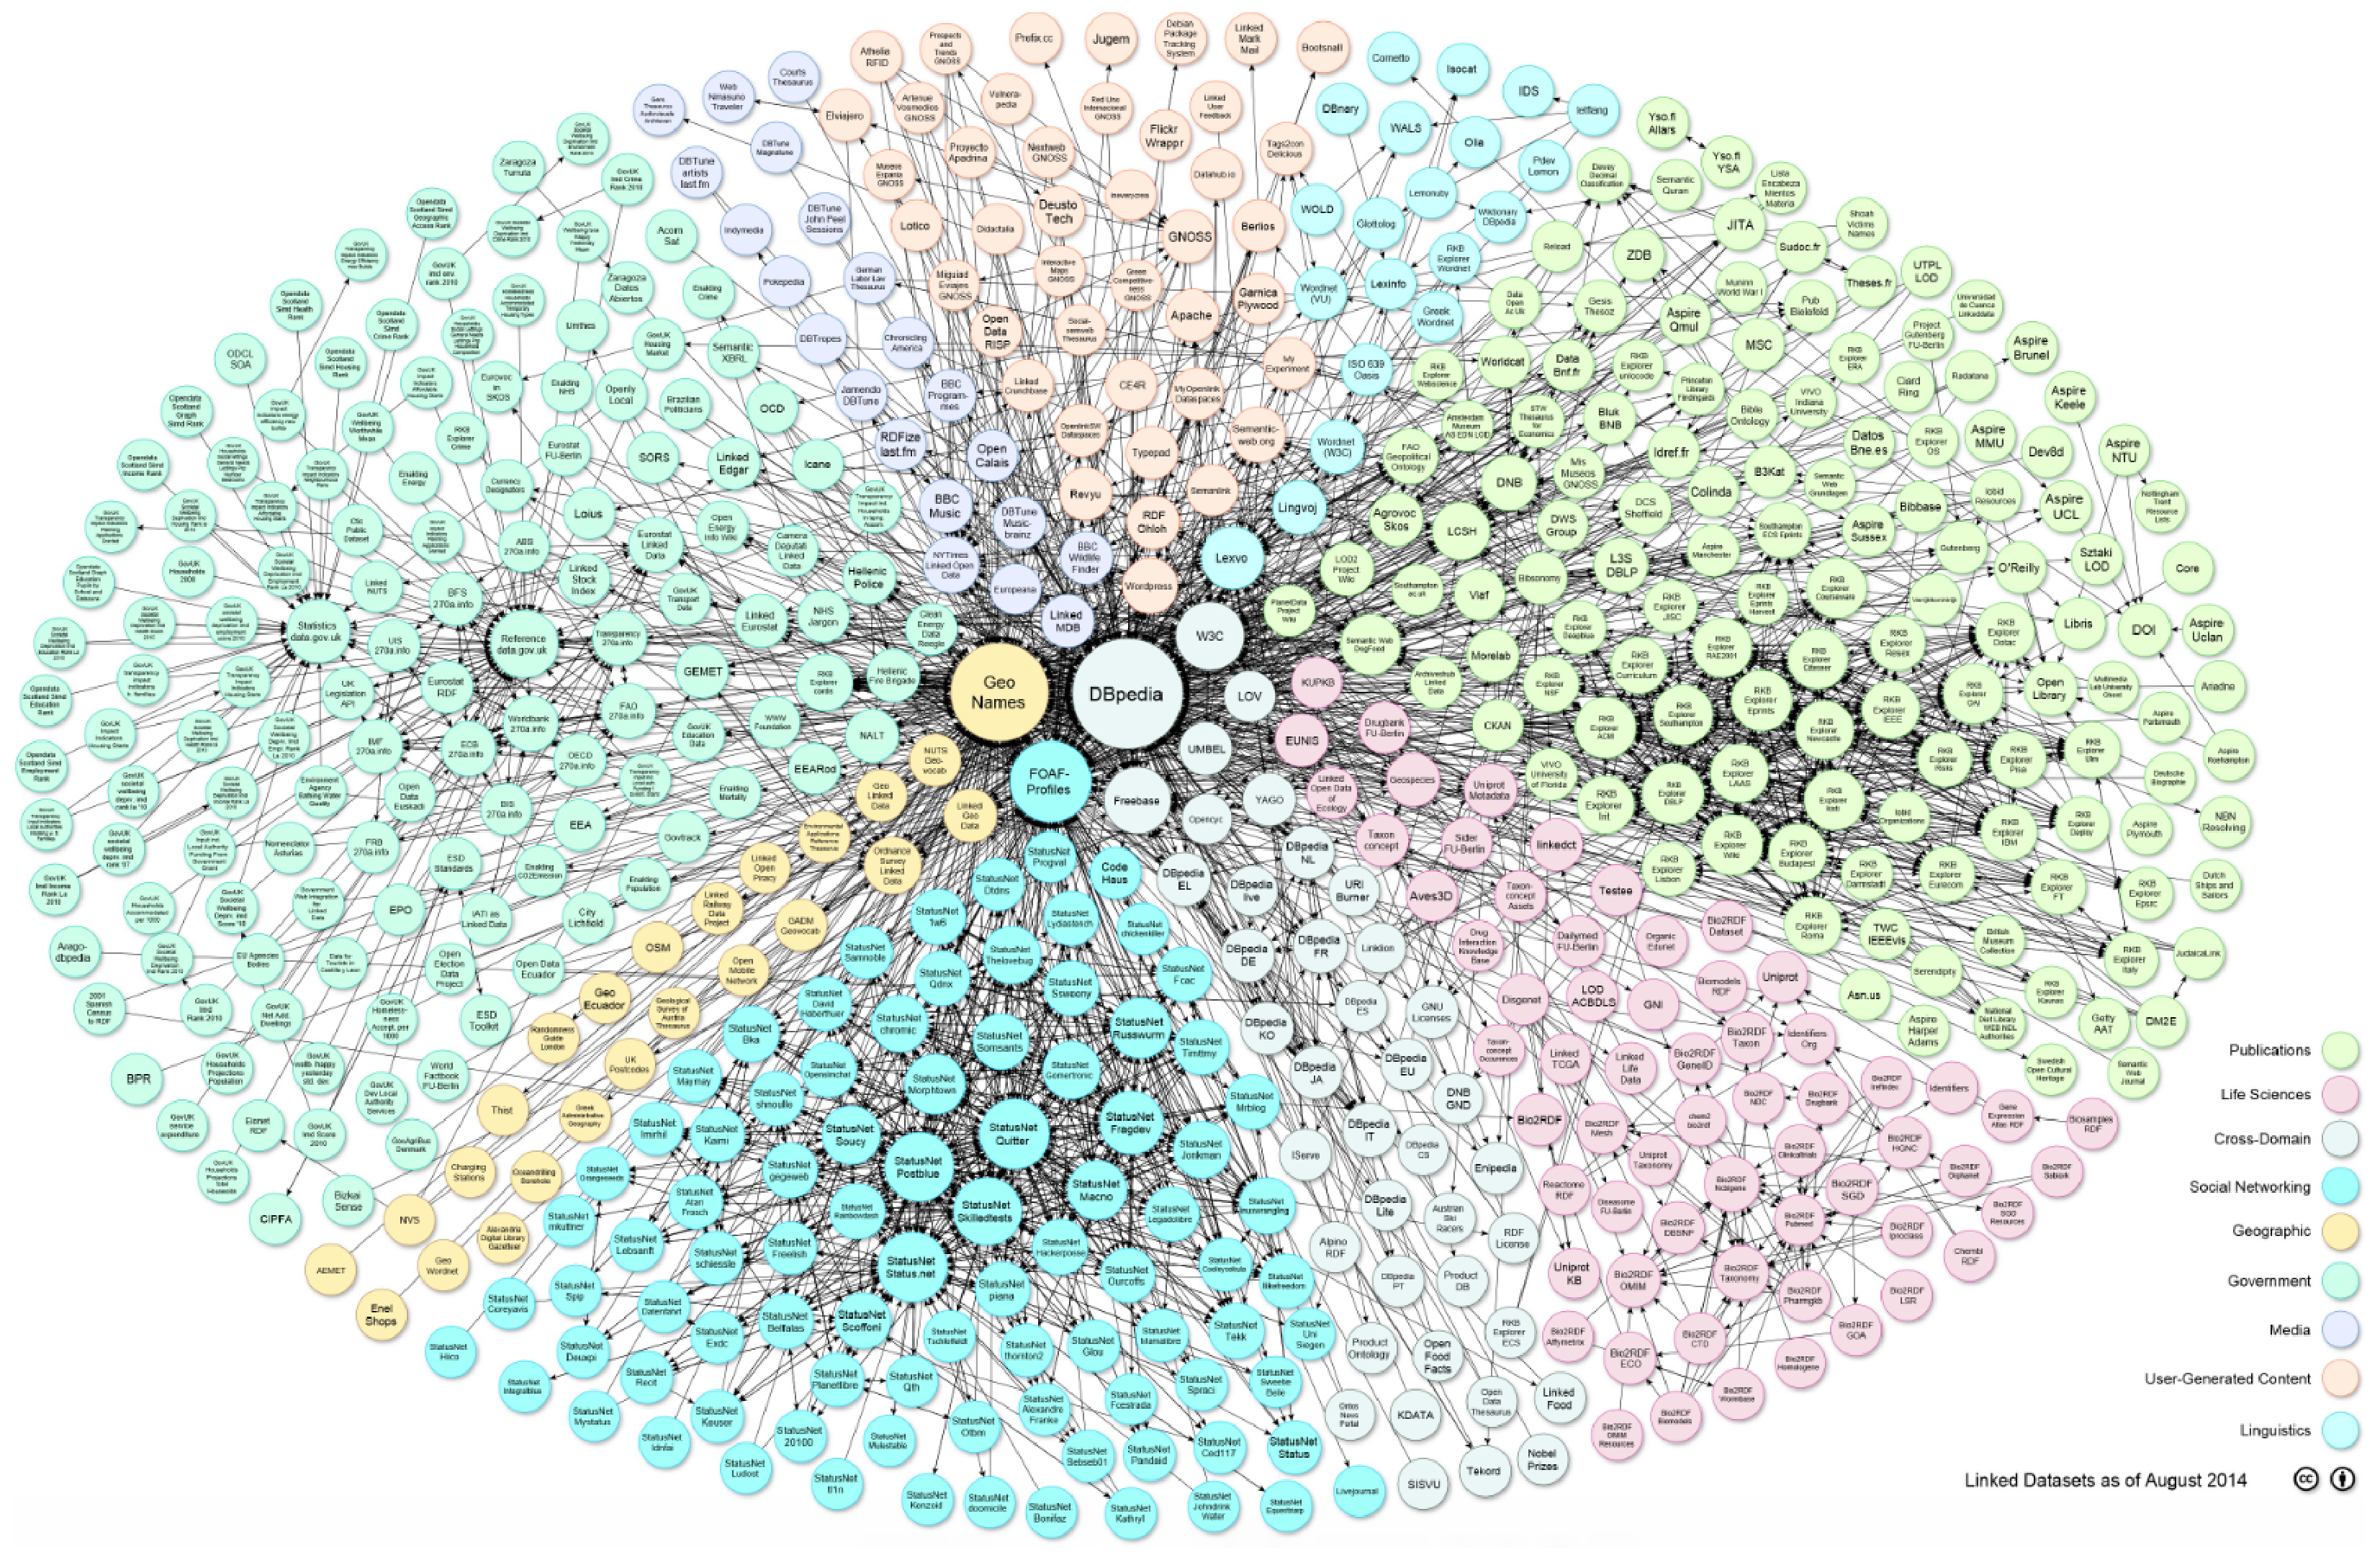
\includegraphics[width=\textwidth]{img/lodcloud.eps}}
\caption{Linked Open Data Cloud, Srpen 2014}
\label{obr:lodcloud}
\end{figure}

\section{Výhody a přínosy otevřených dat a principů Linked data}

\subsection*{Obecné výhody otevřených dat}

\begin{enumerate}
\item Zapojení uživatelů - kontrola, návrhy ke zlepšení dat   
\item Zvýšení transparentnosti vydavatele dat, boj s korupcí
\item Kvalitnější veřejná služba, lepší prezentace subjektu
\item Zvýšení efektivity, úspora nákladů, méně chyb
\item Méně žádostí o data podle zákona č. 106/1999 Sb.\cite{z106} 
\item Široké možnosti dalšího využití - analýzy, statistiky, vizualizace
\end{enumerate}

\subsection*{Výhody principů Linked Data}

\begin{enumerate}
\item Sdílená, rozšiřitelná a snadno znovu použitelná data   
\item Data jsou začleněna do kontextu, resp. lze se odkazovat přímo na data
\item Data jsou propojena s dalšími relevantními daty, informační hodnota dat je tedy tím větší, čím více mají vazeb
\item Standardizované formáty pro publikaci
\end{enumerate}

\newpage

\section{RDF (Resource Description Framework)}
\label{sec:RDF}

Formát RDF byl vyvinut za účelem snadného strojového zpracování a propojování dat. Jedná se o čistě abstraktní formát udávající, jak data popisovat. Nezabývá se tedy konkrétní podobou výsledných dat. 

Základním stavebním kamenem RDF je tvrzení, resp. trojice: \textbf{Subjekt - Predikát - Objekt} (viz Obr. \ref{obr:rdf_basic}). Subjektem je míněn zdroj, který popisujeme. Predikát je vlastnost, která o objektu něco tvrdí. Objekt je hodnota dané vlastnosti. Jednotlivé trojice mohou na sebe navazovat a vytvořit tak orientovaný graf.

\begin{figure}[h]
\centerline{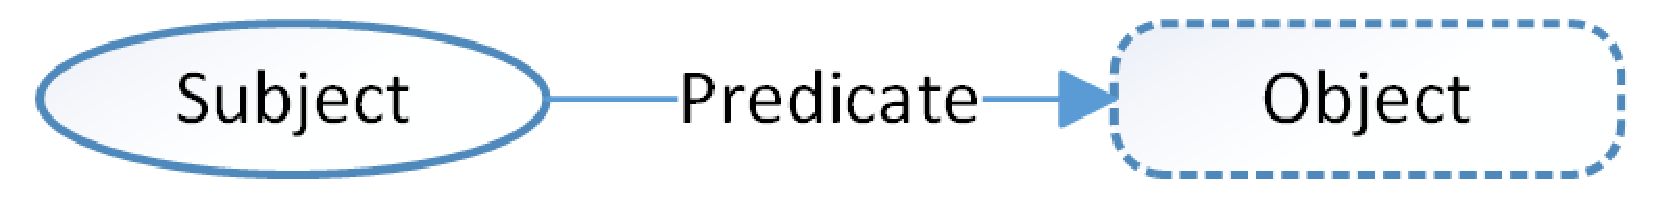
\includegraphics[width=110mm]{img/rdf_basic.eps}}
\caption{Základní RDF trojice}
\label{obr:rdf_basic}
\end{figure}

\subsection*{Nyní definujeme několik pravidel a doporučení pro popisování dat v RDF}

\begin{enumerate}
\item Každý subjekt je jednoznačně identifikován pomocí URI, nebo je označen jako anonymní\footnote{Subjekty, příp. objekty lze označit jako anonymní, resp. pomocí tzv. Blank node. Na anonymní subjekty, resp. objekty ale nelze přímo přistupovat. Používají se typicky k zapouzdření, či jako kontejnery jiných objektů.} 
\item Objektem je buď hodnota (literál), odkaz na subjekt (resource), nebo je označen jako anonymní
\item Pro každý subjekt je specifikován jeho typ (třída) formou URI
\item Každému predikátu je přiřazen také jeho typ formou URI
\item Jednotlivé URI z bodů 3, 4 by měly odkazovat na konkrétní slovníky tříd a predikátů, resp. ontologie
\end{enumerate}

Na obr. \ref{obr:rdf_graph} vidíme příklad jednoduchého grafu ve formátu RDF (aplikována pravidla 1 a 2). Popisuje 3 subjekty a přiřazuje jim konkrétní vlastnosti. Vidíme, že každý subjekt je identifikován vlastním URI. Díky tomu mohou subjekty na sebe odkazovat. Jednotlivé trojice by pak vypadaly takto:

\begin{enumerate}
\item \textit{http://rsmluv.cz/contract/42/1 - Název - Softwarová zakázka}   
\item \textit{http://rsmluv.cz/contract/42/1 - Smluví strana - rsmluv.cz/party/420}
\item \textit{http://rsmluv.cz/party/420 - Název - Magistrát HMP}
\item \textit{http://rsmluv.cz/party/420 - Adresa - rsmluv.cz/party/420/address}
\item \textit{http://rsmluv.cz/party/420/address - Ulice - Staroměstké nám. 4}
\end{enumerate}

\begin{figure}[h]
\centerline{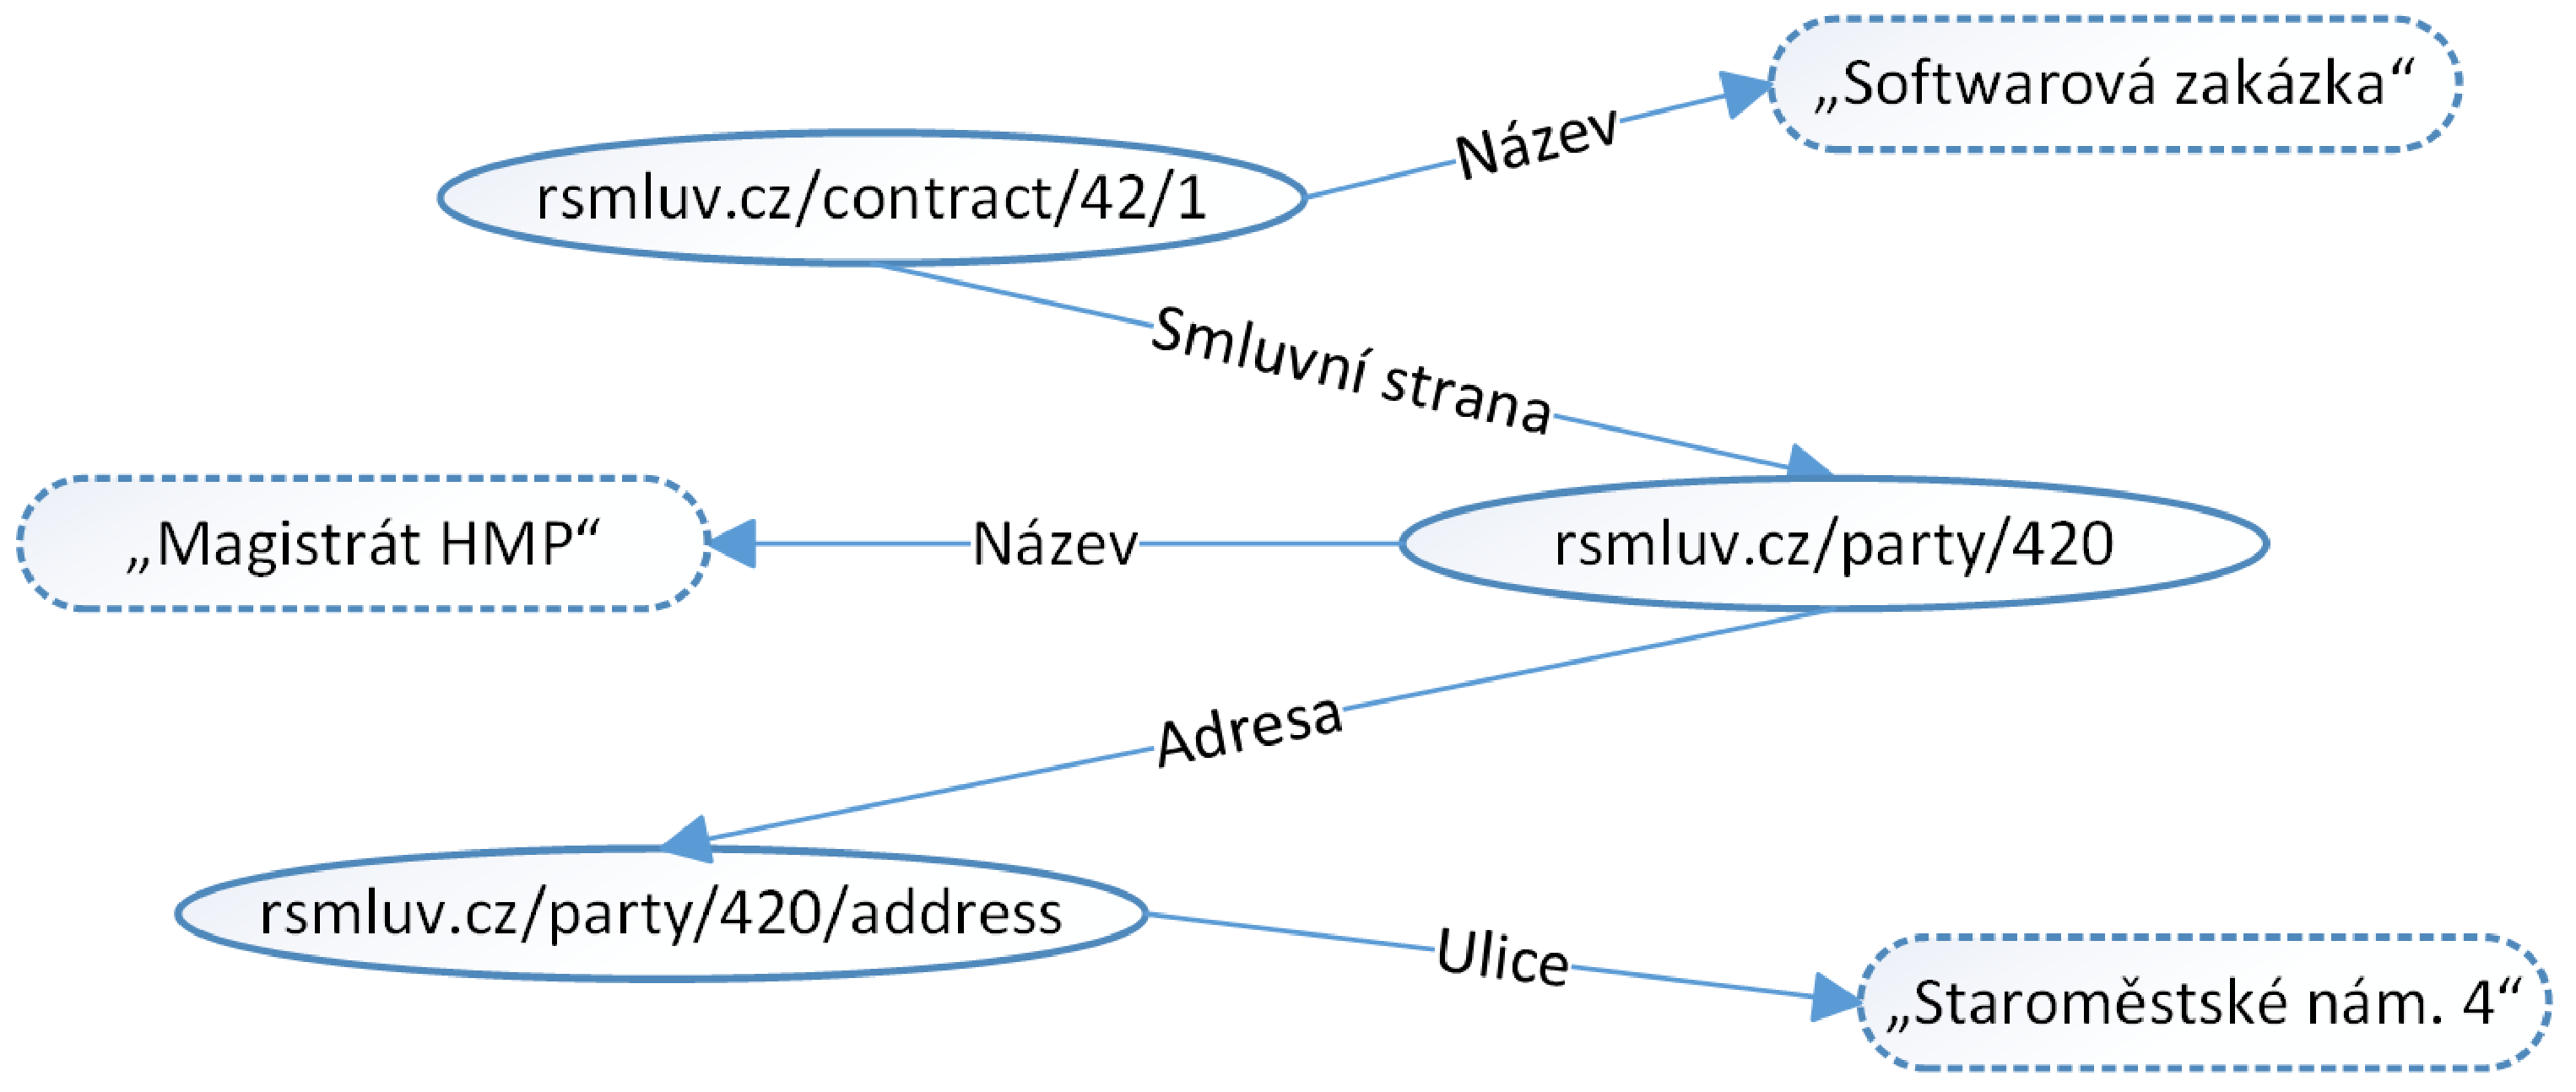
\includegraphics[width=\textwidth]{img/rdf_graph.eps}}
\caption{Jednoduchý RDF graf}
\label{obr:rdf_graph}
\end{figure}

Ze zmíněného příkladu ale není zřejmý význam, resp. sémantika jednotlivých subjektů a predikátů. Je tedy důležité jim přiřadit konkrétní typy. Každý typ by měl být popsaný v konkrétním slovníku tříd a predikátů. Takovéto slovníky nazýváme ontologiemi. Na obr. \ref{obr:rdf_graphWithOntology} vidíme zmíněný příklad rozšířený o přiřazené typy (aplikována pravidla 3, 4, 5)\footnote{Pro zapisování typů se kvůli úspornosti používají prefixy definované typicky na začátku dokumentu.}.

\begin{figure}[h]
\centerline{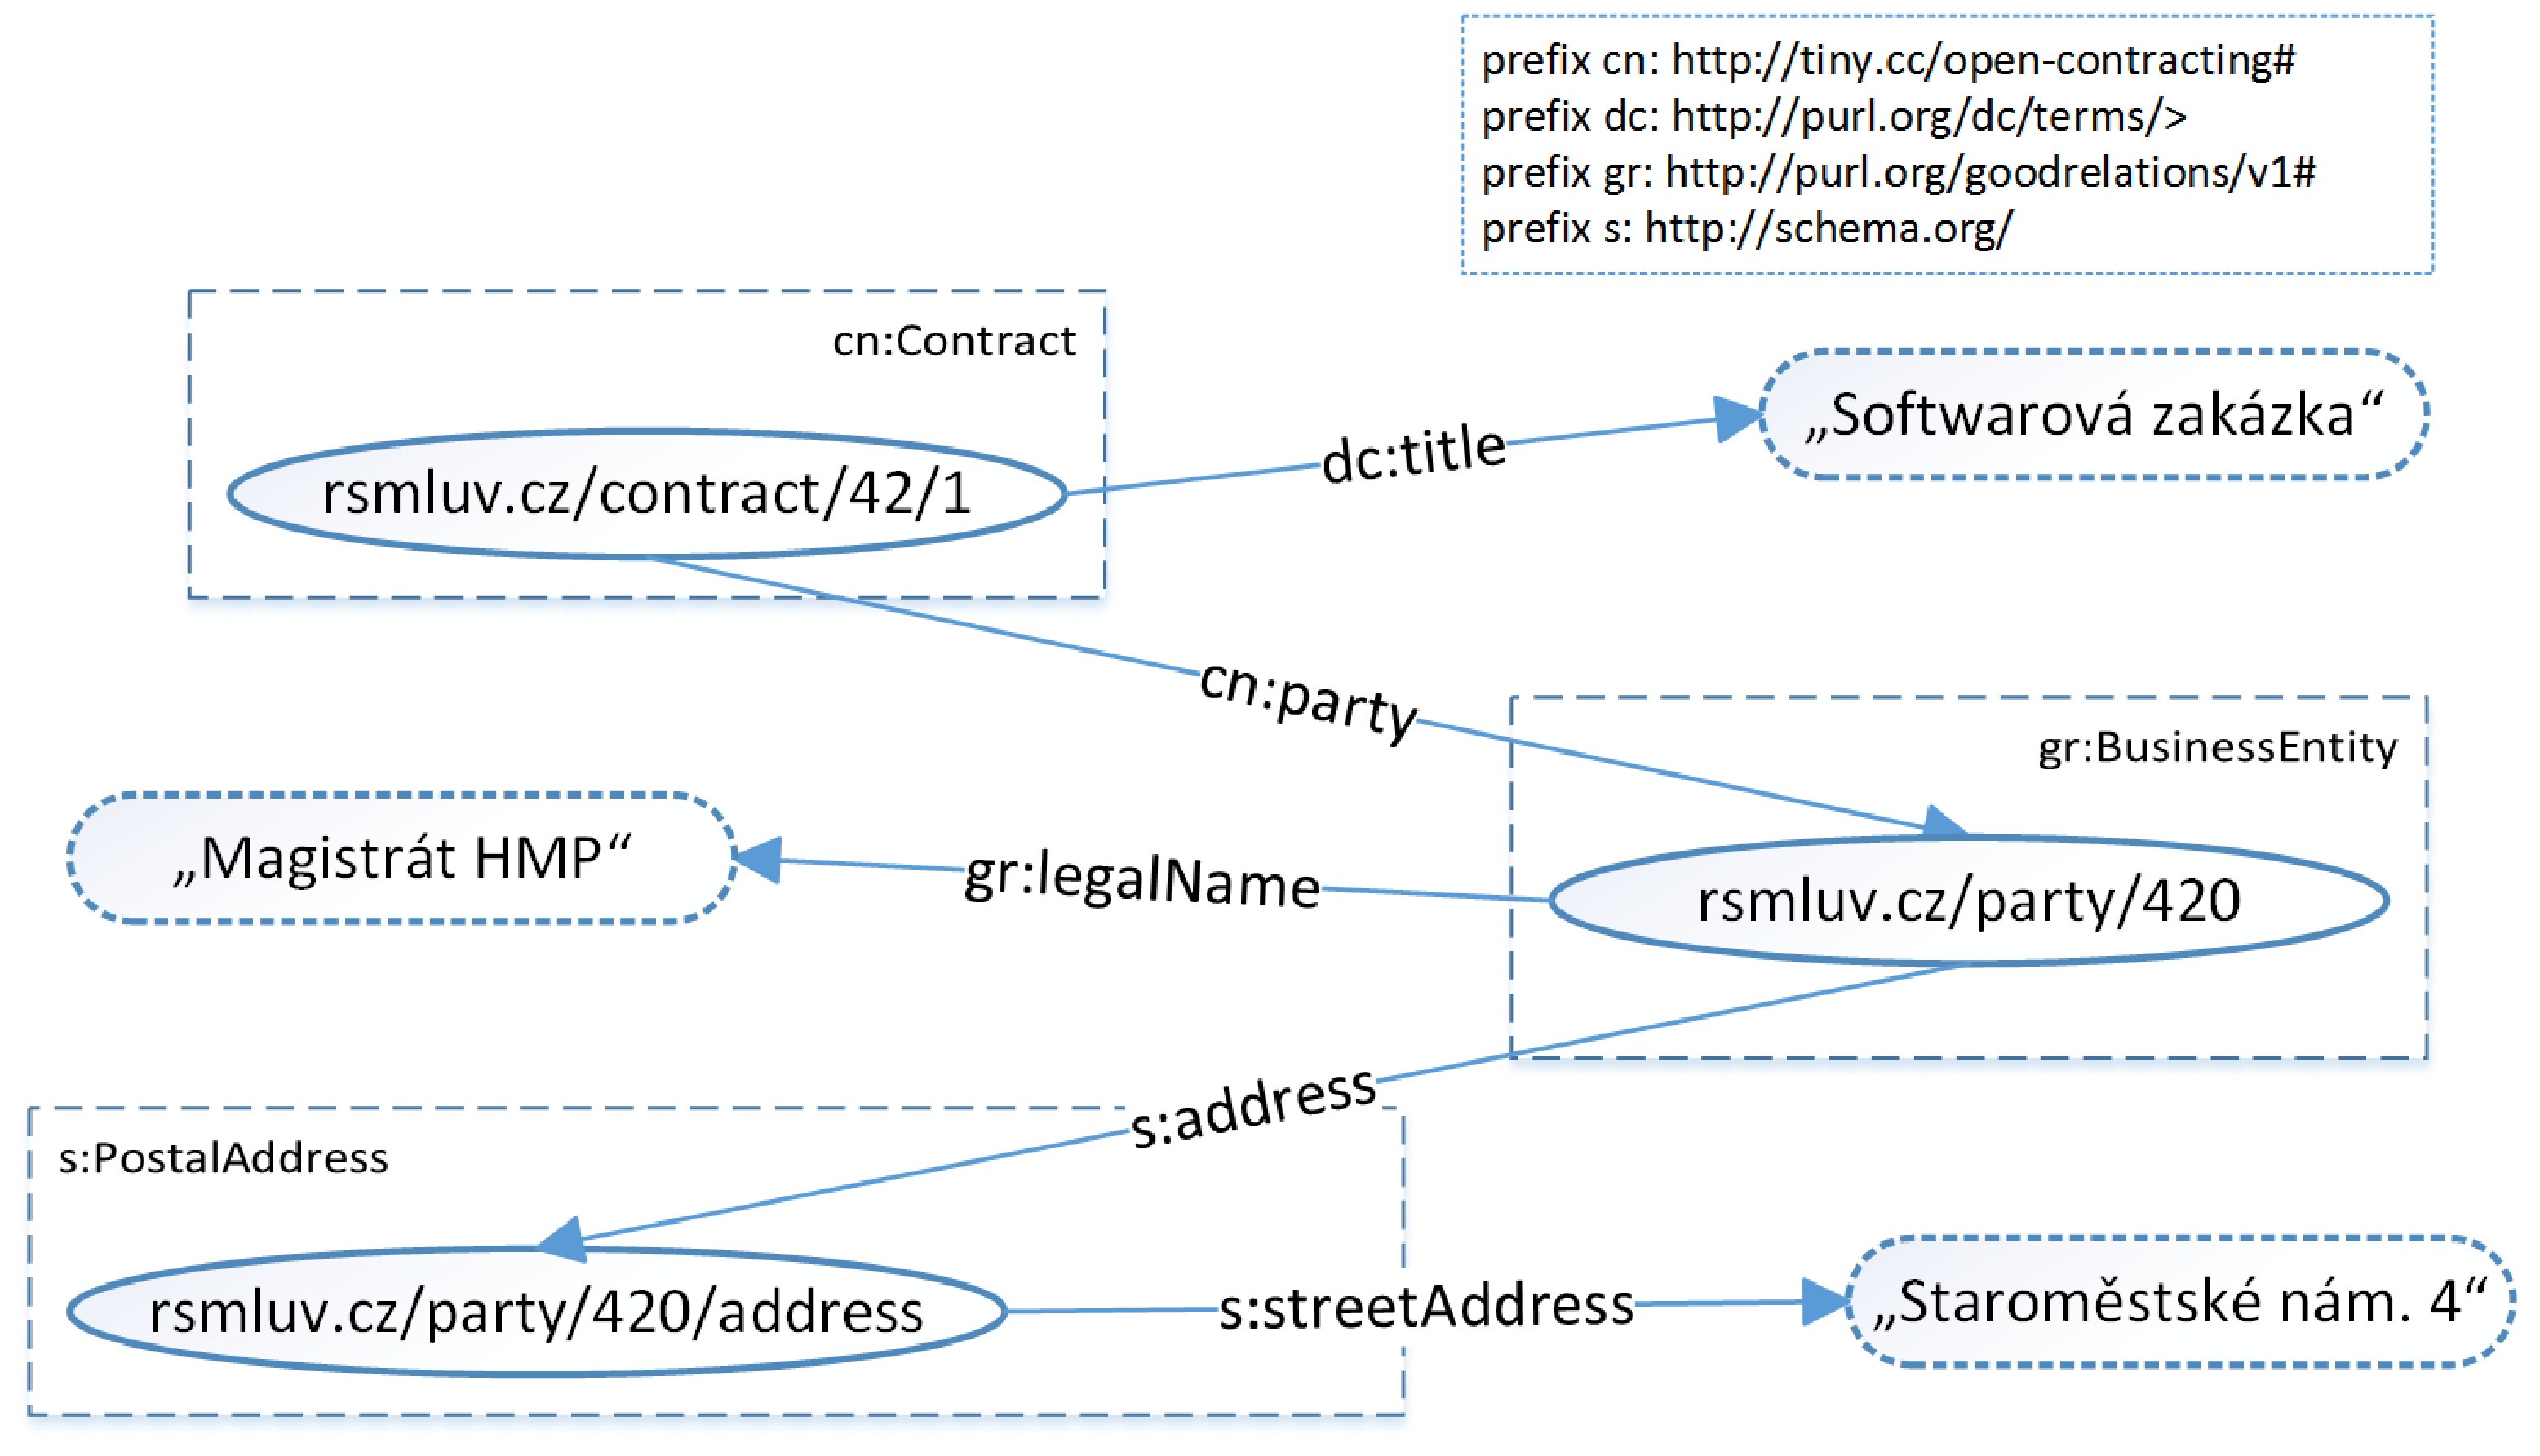
\includegraphics[width=\textwidth]{img/rdf_graphWithOntology.eps}}
\caption{RDF graf s přiřazenými typy}
\label{obr:rdf_graphWithOntology}
\end{figure}

\newpage

\section{RDF Ontologie}

Pod pojmem ontologie si můžeme představit sadu termínů popisujících určitou věcnou oblast. V případě popisování RDF dat definujeme slovník tříd a vlastností (predikátů), které mohou uživatelé ve svých datech používat.

Konkrétní ontologii nelze chápat jako striktně vyžadovaný standard, ale spíše jako sadu doporučení. Buď využijeme k popisu dat nějakou z řady již existujících ontologií, nebo můžeme vytvořit ontologii vlastní. Přesto ale chceme, aby se již existující ontologie používaly co nejvíce. Přínosem je hlavně to, že aplikace a nástroje implementované nad známými ontologiemi budou schopné automaticky rozpoznat naše data\footnote{Mezi všeobecně známé ontologie patří např. DublinCore\cite{dc}, Friend-of-a-Friend\cite{foaf} nebo Schema\cite{schema}. Existuje také katalog ontologií\cite{lov}}. 

Základními jazyky pro modelování RDF dat jsou Web Ontology Language (OWL)\cite{OWL} a RDF Schema (RDFS)\cite{RdfSchema}. Konkrétní specifikace se provádí opět ve formátu RDF a je publikována pod vlastním URI.

Mezi základní výrazové prostředky jazyka OWL a RDFS patří:

\begin{itemize}
\item \textit{owl:Class} - typ entity třída
\item \textit{owl:ObjectProperty} - typ entity vlastnost
\item \textit{owl:FunctionalProperty} - typ jedinečná vlastnost (nemůže se opakovat)
\item \textit{owl:unionOf} - jeden typ třídy z výčtu musí být vyplněn 
\item \textit{owl:equivalentClass} - definuje, že se jedná o třídu odpovídající jiné třídě
\item \textit{owl:equivalentProperty} - definuje, že se jedná o vlastnost odpovídající jiné vlastnosti
\item \textit{rdfs:label} - popis třídy/vlastnosti
\item \textit{rdfs:comment} - komentář třídy/vlastnosti
\item \textit{rdfs:domain} - požadovaný  typ domény třídy/vlastnosti
\item \textit{rdfs:range} - požadovaný rozsah typů třídy/vlastnosti
\item \textit{rdfs:isDefinedBy} - definice zdroje třídy/vlastnosti
\item \textit{rdfs:subClassOf} - definice, že se jedná o podtřídu určité třídy  
\item \textit{rdfs:subPropertyOf} - definice, že se jedná o podvlastnost určité vlastnosti  
\end{itemize}

Na obr. \ref{obr:rdf_ontologyClass} vidíme příklad ontologie třídy Contract. Ontologie nám říká, že se jedná o třídu (typ owl:Class) s názvem Smlouva (rdfs:label), která je podtřídou (rdfs:subClassOf) třídy Document a je definovaná (rdfs:isDefinedBy) v ontologii http://tiny.cc/open-contracting. Kdokoli pak bude zpracovávat entitu označenou tímto typem, tak díky přiřazené ontologii bude schopen určit, že se jedná o smlouvu.

\begin{figure}[h]
\centerline{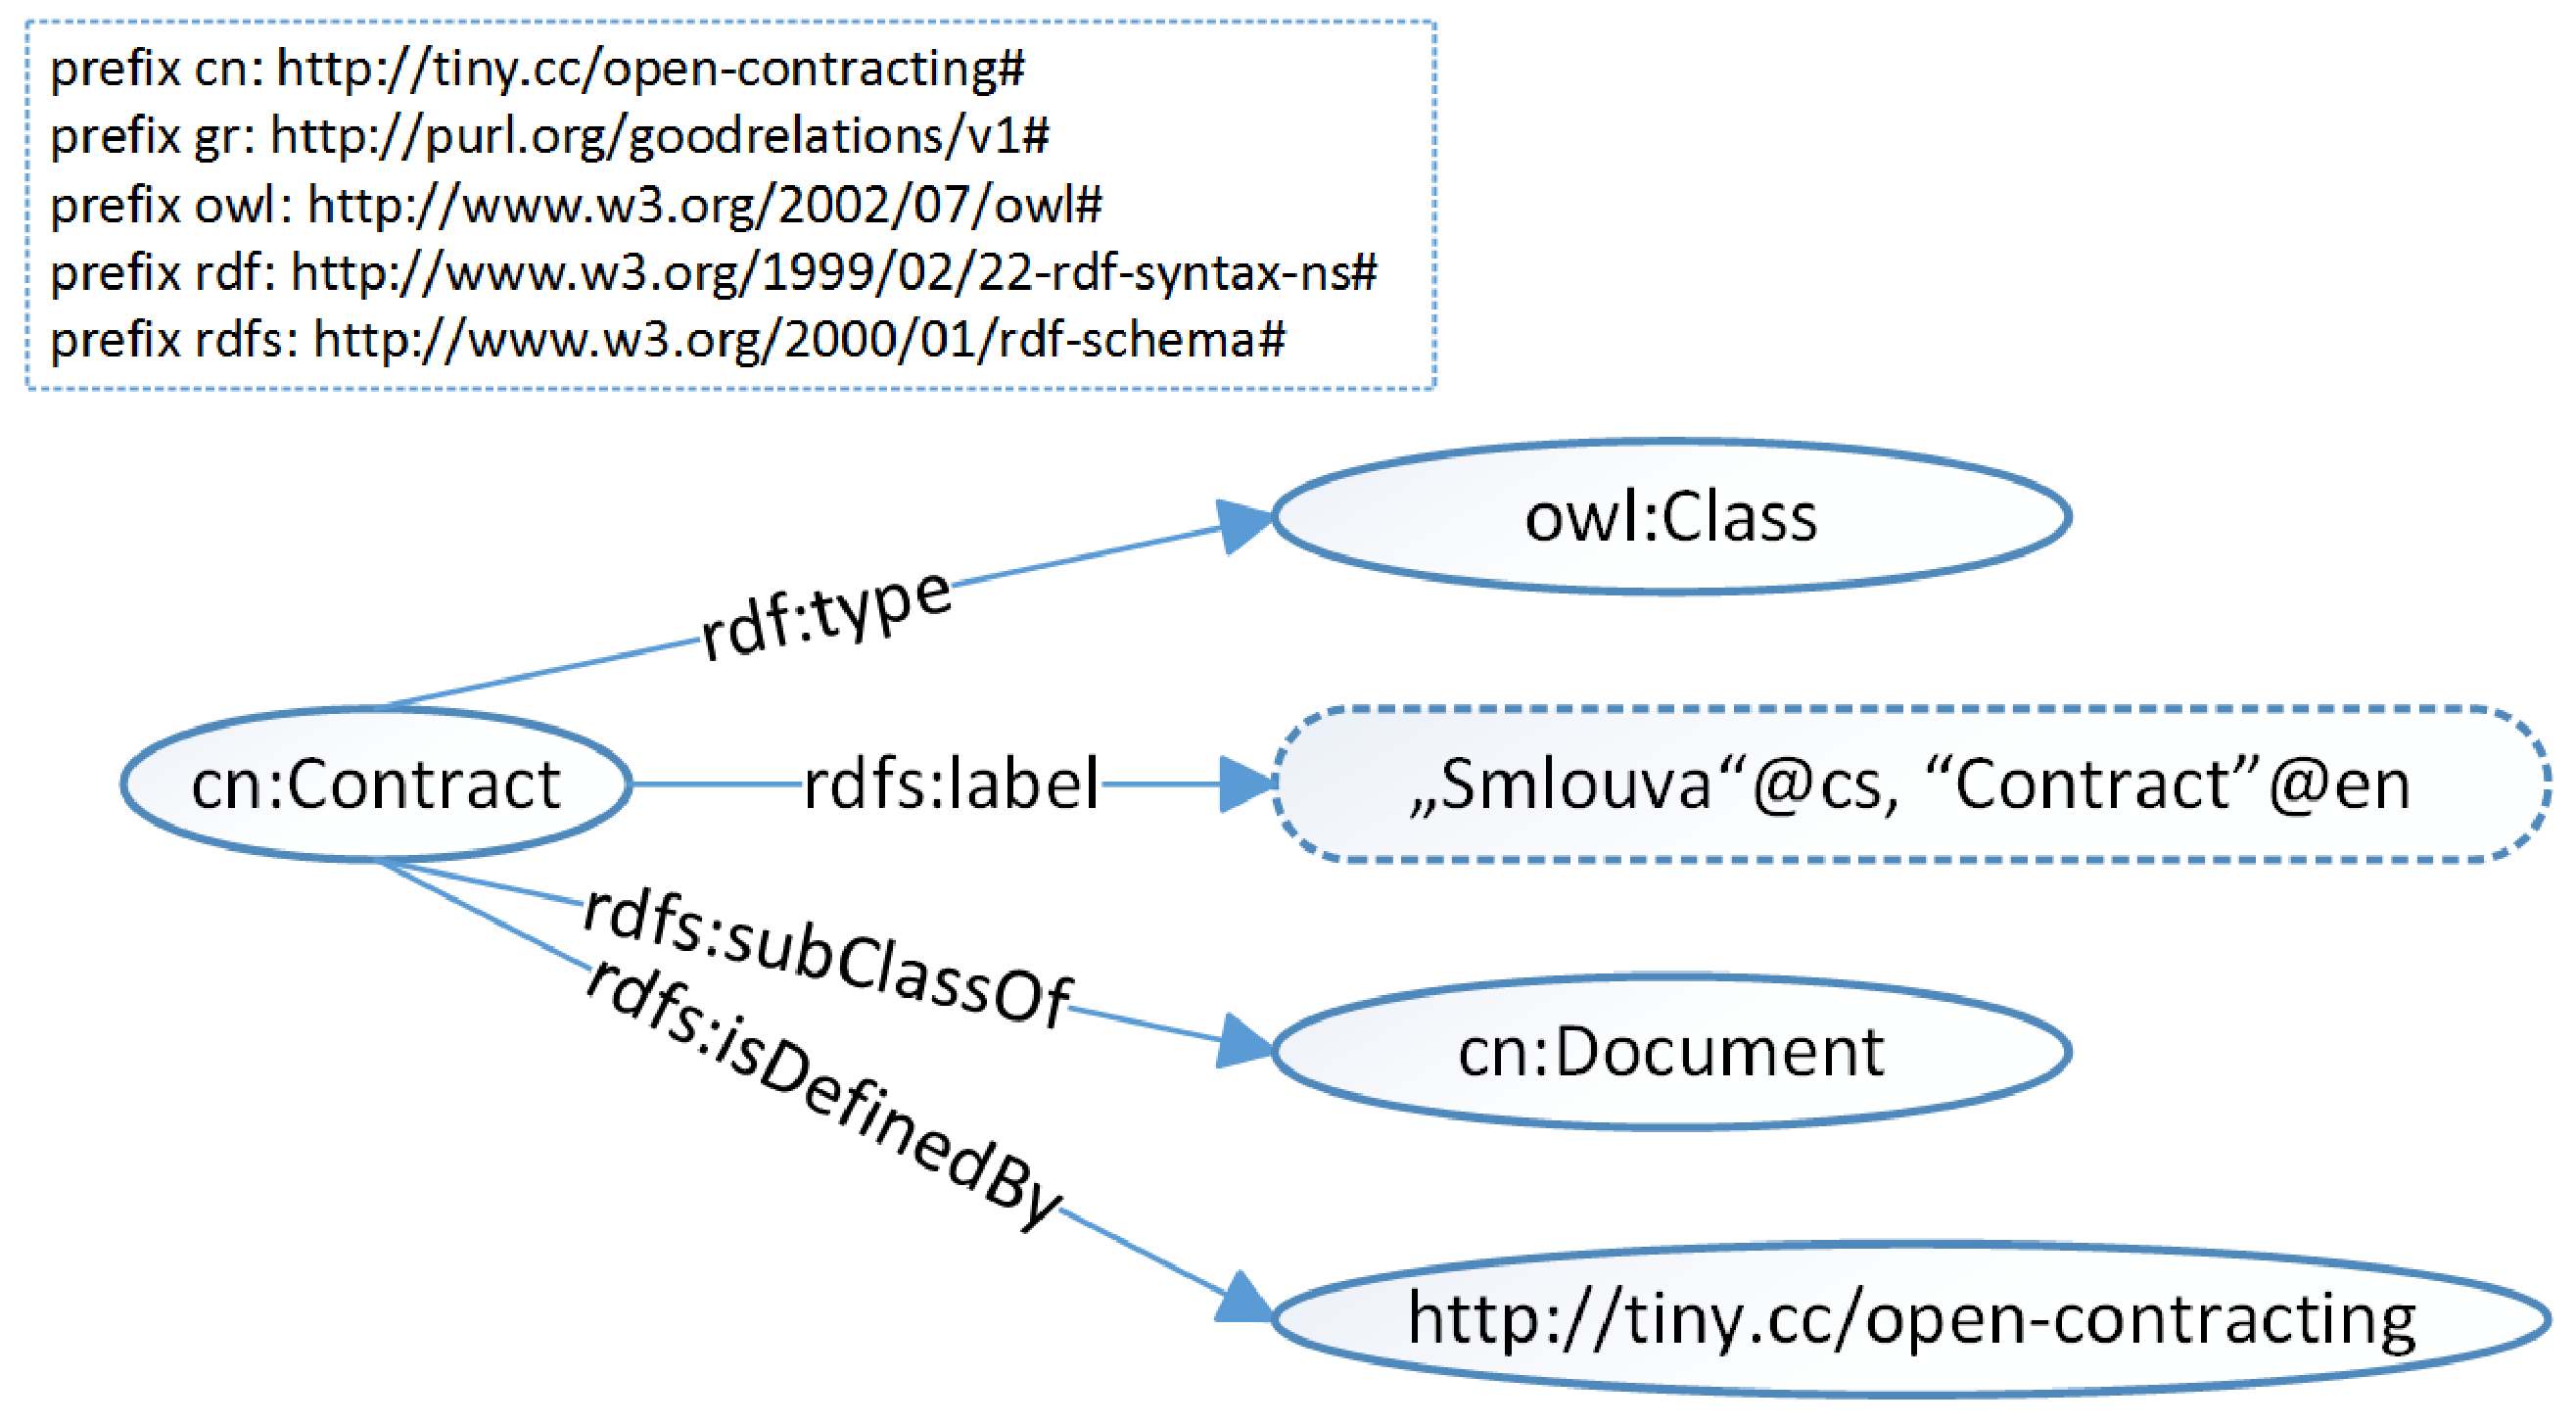
\includegraphics[width=\textwidth]{img/rdf_ontologyClass.eps}}
\caption{Ontologie třídy \textit{Contract}}
\label{obr:rdf_ontologyClass}
\end{figure}

\subsection{Propojování se souvisejícími entitami}

Díky RDF můžeme data reprezentovat jako orientovaný graf. Otázka tedy zní, zdali lze propojovat grafy mezi sebou. Ve formátu RDF je to velmi jednoduché. Jako objekt predikátu stačí položit subjekt z jiného grafu. Díky URI identifikaci entit tedy není rozdílem, zdali je cílovým subjektem entita v lokálních datech, nebo entita cizí.  

V rámci propojování dat s jinými datasety však není neobvyklé, že stejné entity jsou reprezentované v různých datasetech pod vlastními URI. Je tedy třeba vyjádřit, že se jedná o data reprezentující stejné entity. V jazyku OWL za tímto účelem existuje predikát sameAs, kterým můžeme definovat odpovídající si entity (viz Obr. \ref{obr:rdf_ontologyLinks}).

\begin{figure}[h]
\centerline{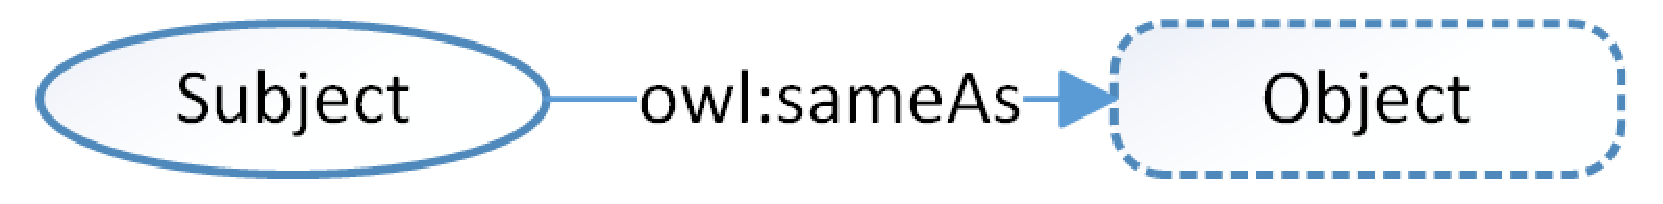
\includegraphics[width=110mm]{img/rdf_ontologyLinks.eps}}
\caption{Odpovídající si entity}
\label{obr:rdf_ontologyLinks}
\end{figure}

\newpage

\section{Publikace}

V minulých kapitolách bylo řečeno, jak popisovat data pomocí RDF. Jednalo se o sémantický popis. Pokud však data chceme publikovat, je třeba konkrétního datového formátu, který definuje syntaxi, resp. jak RDF data serializovat. Takových formátů existuje celá řada, např.:

\begin{itemize}
\item \textbf{N-Triples\cite{N-Triples}} - nejjednodušší serializace RDF grafu v podobě výčtu trojic
\item \textbf{N-Quads\cite{N-Quads}} - rozšíření pro N-Triples s možností zaznamenat více grafů
\item \textbf{RDF/XML\cite{RDF/XML}} - RDF graf serializovaný do XML, využívající prefixového zápisu
\item \textbf{Turtle\cite{Turtle}} - úsporný textový formát s možností komprese trojic, využívající prefixových zápisů
\item \textbf{Trig\cite{Trig}} - rozšíření Turtle pro použití nad více grafy
\item \textbf{RDFa\cite{RDFa}} - serializace RDF do (X)HTML dokumentů, využívající prefixového zápisu
\item \textbf{JSON-LD\cite{JSON-LD}} - specifický zápis RDF grafu, využívající mapování položek JSON dokumentu na RDF ontologie
\end{itemize}

Pro potřeby této práce si vystačíme s formáty N-Triples, Turtle a JSON-LD. Vysvětlíme si je na příkladech. Jako data k serializaci použijeme příklad z obr. \ref{obr:rdf_graphWithOntology}.

\subsection{Příklad dat serializovaných ve formátu N-Triples}

Serializace RDF dat do N-Triples je velmi jednoduchá. Jedná se o seznam trojic oddělených tečkou. Každá trojice je uvedena na vlastním řádku. Tento formát nepoužívá prefixové zkracování URI. Je vhodný pro proudové zpracování velkého množství dat (viz Obr \ref{lst:ntriples_example})\footnote{Trojice nejsou z důvodu přehlednosti uvedeny na samostatných řádcích}.\\

\lstinputlisting[label=lst:ntriples_example,caption=Příklad RDF dat - N-Triples, language=XML]{code/ntriples_example.nt}

\subsection{Příklad dat serializovaných ve formátu Turtle}

Formát Turtle umožňuje zkracování URI pomocí prefixů. Umožňuje také zkracovat zápis tím, že nemusíme zapisovat opakující se subjekt. Jednotlivé dvojice predikát-hodnota lze tak přehledně mít u jednoho subjektu. Oddělovačem mezi dvojicemi v rámci subjektu je středník, blok informací o daném subjektu je zakončený tečkou. Pro definování typu subjektu se může použít klíčové slovo \uv{a}, namísto predikátu rdf:type. Výhodou formátu je úspornost a velmi dobrá lidská čitelnost (viz Kód \ref{lst:turtle_example}).\\

\lstinputlisting[label=lst:turtle_example, caption=Příklad RDF dat - Turtle, language=XML]{code/turtle_example.ttl}

Díky dobré čitelnosti, se formát Turtle hojně používá pro zapisování ontologií. V kódu \ref{lst:turtleOntology_example} vidíme znázorněnou jednoduchou ontologii. Popisuje 2 objekty. Prvním je třída Contract (typ owl:Class). Definuje, že se jedná o smlouvu, je podtřídou (rdfs:subClassOf) třídy Document a je definována v ontologii (rdfs:DefinedBy) http://tiny.cc/open-contracting. Je to serializovaný zápis ontologie z obr. \ref{obr:rdf_ontologyClass}. Druhým objektem je vlastnost party (typ owl:ObjectProperty). V predikátu rdfs:domain je specifikováno, že vlastnost party může být použita u třech tříd, a to Contract, Order nebo Invoice. Predikát rdfs:range znamená, že očekávaný přiřazený objekt je typu gr:BusinessEntity.\\

\lstinputlisting[label=lst:turtleOntology_example, caption=Příklad RDF Ontologie - Turtle, language=XML]{code/turtleOntology_example.ttl}

\subsection{Příklad dat serializovaných ve formátu JSON-LD}

JSON-LD je jedním z poměrně nových formátů pro serializaci RDF. Jednou z motivací k vzniku byla snaha využít hojně využívané JSON dokumenty v dnešních aplikacích a co možná nejefektivněji z nich vytvořit RDF data.

Uveďme si modelový příklad. V kódu \ref{lst:json_example} jsou ne-RDF data ve formátu JSON. Jsou validní vůči nějakému JSON Schématu a používají se v konkrétních aplikacích.  

V kódu \ref{lst:jsonld_example} máme stejná data v RDF podobě. Jak je vidět, jednotlivým objektům je přiřazen typ a URI. Použije se k tomu klíčových slov @type, resp. @id. K dokumentu je také přiložen kontext (klíčové slovo @context), kde se definuje mapování vlastností původního JSON dokumentu na RDF ontologie. Zachovává se tedy původní struktura JSON dokumentu. Kontext však nemusí být přímo součástí JSON-LD dokumentu, lze se na něj odkazovat. 

Výsledkem tedy může být JSON-LD soubor (viz Kód \ref{lst:jsonldWithContext_example}). Jedná se tedy pouze o lehce rozšířený původní JSON dokument. Z tohoto důvodu bude pravděpodobně takový dokument nadále validní vůči JSON Schématu a použitelný ve stávajících aplikacích. Přináší však tu výhodu, že se zároveň jedná o RDF data.

\newpage

\lstinputlisting[label=lst:json_example, caption=Obyčejný JSON dokument, language=XML]{code/json_example.json}

\lstinputlisting[label=lst:jsonld_example, caption=Příklad RDF dat - JSON-LD, language=XML]{code/jsonld_example.jsonld}

\lstinputlisting[label=lst:jsonldWithContext_example, caption=Příklad RDF dat - JSON-LD s Contextem, language=XML]{code/jsonldWithContext_example.jsonld}